\documentclass[paper=a4, fontsize=10pt]{scrartcl}

\usepackage{physics-math}

\usepackage{natbib}
\usepackage{subcaption}

\linespread{1.05}


\title{Master Praktikum - Magnetisation}
\subtitle{Advanced lab course in
  physics for Master students - experiment: magnetisation studies}
\author{Alex Kreuzer - group 12}

\date{\normalsize\today}

\begin{document}

\maketitle
\newpage

\renewcommand{\contentsname}{Table of contents}
\tableofcontents

\pagebreak

\section{Aim of the experiment}

The main goal of this experiment is the measurement of the
magnetisation for two lanthanoids, gadolinium (Gd) and terbium (Te).
Using a \textbf{S}uperconducting \textbf{Qu}antum
\textbf{I}nterference \textbf{D}evice (SQUID), which is a high
sensitive measuring instrument for changes in magnetic flux, and a
platinum thermometer the magnetisation can be measured as a function
of temperature. Additionally the Curie temperature for the materials
can be calculated.


\section{Essential theory}

\subsection{Superconductivity}

For certain materials the material's electric resistance drops to zero
under certain conditions. These materials are called superconductive
materials and focusing on the metallic ones, those can be classified
in type I or type II superconductor. Superconductive metals of type I
show below specific temperatures a drop of electric resistance to
zero. As a result the material will become perfect diamagnetic inside
the material, where an external magnetic field will be suppressed
completely within the solid state device just under the surface
(Meissner effect).


According to the BCS-theory of 1957 superconductivity can be described
by quantum effects. Within this theory a superconductive material can
form so called Cooper pairs, pairs of two electrons with opposite
spin, which form a bosonic particle of zero spin reacting to
Bose-Einstein statistics. Since the bosonic Cooper pairs are
delocalised within the quantum state of the material, the interaction
of the Cooper pairs with the lattice is suppressed and Cooper pairs
can propagate without an electric resistance. Above the critical
temperature $T_C$ a superconductor of type I will rapidly react as a
common conductor with resistance.


Superconductors of type II show similar properties compared to type I
superconductors until they are exposed to a external magnetic field
exceeding a certain strength of magnetic field. Above this lower
critical magnetic field the external field can enter the
superconductive material partially till the superconductive properties
void above an upper critical magnetic field strength. \
subsection{Superconducting Quantum Interference Device -SQUID}


Superconducting devices can be used for highest precision measurement
of very small changes in magnetic fields. In this experiment a SQUID,
superconductive quantum interference device, is used. This device
consists of a superconductive torus with diameter of about half an
millimetre which is disconnected by a thin insulating part. This
particular setup of two (or here one cyclic) superconductors separated
by a thin layer of insulating material is described by the Josephon
effect.


Cooper pairs on both sides of the insulator junction have extended
wave functions overlapping at the junction for a sufficient thin layer
of insulator. A current can pass the insulator due to tunnel effects
of Cooper pairs. One can measure current and voltage at the Josephon
junction, which react on a external magnetic field.


To understand this, one has to consider the magnetic flux. Without any
external field, the magnetic flux of an torus is constant in total.
Since the flux is caused by bonic Cooper pairs, the flux is considered
to be quantized to be a multiple of a the flux of an Cooper pair,
which is called fluxon. Since a Cooper pair consists of two electrons
the magnetic flux of a single fluxon, the flux quantum, can be
calculated in BSC theory to be
$\Phi_0=h/2e\approx 2,07 \cdot 10^{-15}~$Vs where $h$ is Planck's
constant and $e$ the electron's charge.


Under conditions of superconductivity the whole magnetic flux within
the SQUID torus is constant and a multiple of integer $n$ of $\Phi_0$
$$\Phi_{ext}+I\cdot L = n\cdot\Phi_0 = \text{const}$$
where $L$ is the conductivity of the torus with current $I$. An
external magnetic field causes a flux $\Phi_{ext}$, where a change in
magnetic field causes Cooper pairs to generate or degenerate.


A magnetic flux across the SQUID causes an electric current $I$ which
is compensated by multiple fluxon. The superconductive surrent is due
to this proportional to the change of magnetic field. Since the change
of an external magnetic field can only be compensated by an integer
multiple of $\Phi_0$. Is the electric current $I$ aboce a critical
current $I_C$ the superconductivity voids and one can measure a
voltage at the junction.


The SQUID consist of yttrium-barium-copper-oxide and the insulating
part is implemented by for grain boundaries, where a grain boundary is
an interface between two crystal parts ("grains") in a polycrystalline
material. These boundaries are defects in the crystal structure,which
decreases the electrical and thermal conductivity at this point. The
setup allows only one single fluxon of $\Phi_0$ to cross the junction
leading to a current. This means, that only one fluxon can compensate
the change of an external magnetic field before $I_C$ is reached.


The SQUID is coupled via magnetic induction with high-frequency
AC-field of a LRC circuit. The LRC circuit has a resonance frequency
between $100~$MHz an $1~$GHz and can induce a AC-current within the
SQUID via the flux at the Josephon junction leading to a periodic
alternating change of superconductive and ohmic conductivity. In ohmic
conductivity state the LRC circuit transfers energy into the SQUID
leading to ohmic heating of the SQUID and a reduced voltage at the LRC
circuit, which is damped. The change in voltage by damping can be
measured and thus the current within the SQUID torus. The coupled RLC
circuit is used as a pump device for the squid. Figure \ref{fig:SQUID}
shows the schematic principle of the SQUID and circuit.


If the SQUID is exposed to an additional external magnetic field, this
would effect the "pumping process" of the circuit and one would
measure a different voltage curve. This is shown in figure
\ref{fig:SQUID2}.


\begin{figure*}[h!] 
	\centering
	   \begin{subfigure}[t]{0.5\textwidth}
 	       \centering
	       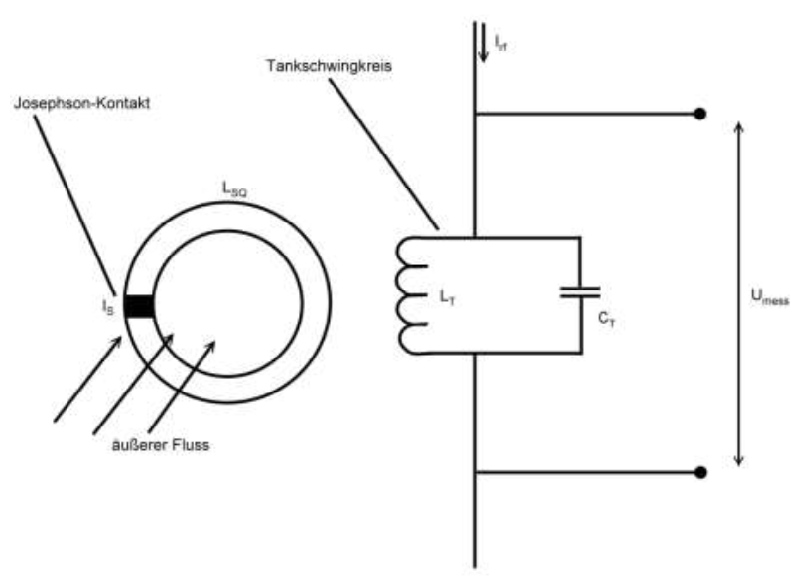
\includegraphics[height=2.5in]{img/SQUID2}
       	       \caption{Schematic depiction of the SQUID torus in
                 profile with the coupled LRC circuit.}
 	       \label{fig:SQUID}
    \end{subfigure}
	  \begin{subfigure}[t]{0.5\textwidth}
	        \centering
	        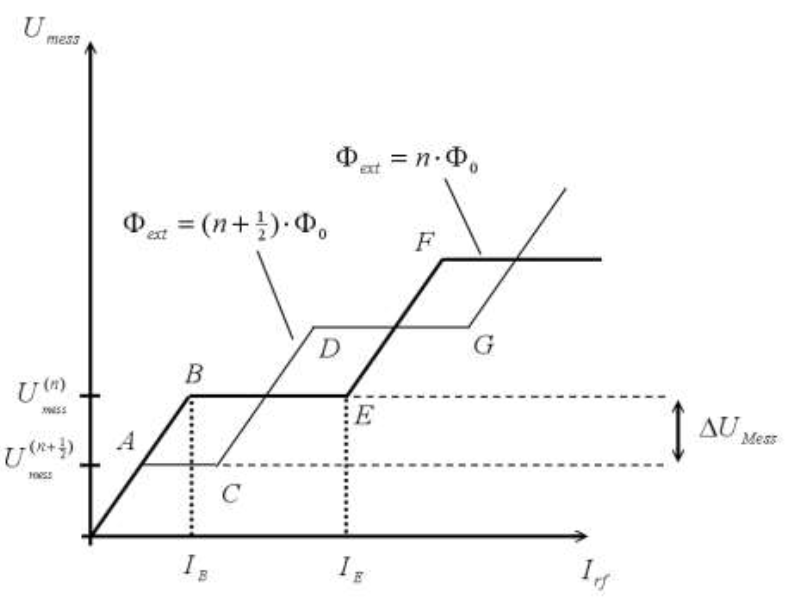
\includegraphics[height=2.6in]{img/SQUID}
 	        \caption{Voltage $U_{mean}$ measured at the LRC
                  circuit as a function of the current $I_{rf}$
                  measured at the superconductive torus.}
	 	\label{fig:SQUID2}
	  \end{subfigure}
          \caption{The principles of SQUID technology for the
            measurement of small magnetic fields. Figures taken from
            \citep{SQUID}}
\end{figure*}

Depending on the external flux, the curve is shifted along the
$I_{rf}$ axis. Figure \ref{fig:SQUID2} shows this effect in case of
$n$ fluxons and $(n+\frac{1}{2})$ fluxons. The strength of the
external AC field of the circuit will affect the scale of the measured
voltage $U_{mean}$. To ensure a precise measurement in the experiment
another coils is used to compensate the flux within the SQUID. The
second coil is proportional to the change of magnetic field.

\newpage

\subsection{Magnetism in solid states}

In this experiment different types of magnetism will be observed
depending of the materials temperature. Therefore a short summary of
the main types of magnetism are introduced here. The magnetic flux
density is given by the magnetic field $H$ via the magnetic
susceptibility $\chi_m$, which is a scalar for small magnetic fields
(otherwise $\chi_m$ is a tensor for higher orders in $H$) and the
permeability constant $\mu_0$

$$B=\mu_0 (1+\chi_m)H$$

A more demonstrative quantity is the relative susceptibility
$\chi_r=\chi_m/\mu_0$. Different types of magnetism lead to different
values of $\chi_r$.


\subsubsection*{Ferromagnetism}


The material's magnetic properties are based on the magnetic moments
of the material's components. In case of lanthnoid materials like Gd
or Tb the relevant particles are the $4f$-orbital and conductive
electrons.

In case of ferromagnetic properties the $4f$-orbitals electron spins
are not distributed randomly, but rather oriented parallel in same
direction to each other forming so called Weiss domains. Exposed to an
external magnetic field the magnetic moments will align in direction
of the external field depending of the fields strength. After the
influence of an external field most of the magnetic moments will keep
the alignment without an external magnetic field depending of the
materials temperature. Above the Curie-temperature $T_C$ the thermal
energy will be enough to destroy the magnetic alignment of the Weiss
domains and the ferromagnetic properties void.

For ferromagnetism the susceptibility reaches high values
($\chi_r\gg1)$ till saturation points depending of the orientation of
the magnetic moments.


\subsubsection*{Antiferromagnetism}

In case of antiferromagnetic properties the magnetic moments are
oriented parallel in opposite direction to each other. Since the
alignment is in opposite direction the resulting macroscopic momentum
is zero. Antiferromagnetic properties are typically observed at very
low temperatures up to the so called Neèl-temperature $T_N$. Above
this temperature the thermal energy will be enough to destroy the
antiferromagnetic order.


\subsubsection*{Paramagnetism}

In case of paramagnetism the magnetic moments are distributes
randomly, that no macroscopic magnetic magnetisation can be observed.
Exposed to an external magnetic field, the single magnetic moments
will align along the external fields in same direction so the magnetic
field inside the material will amplify.


For paramagnetism the relative suceptibility is small and positive
($\chi_r>0$).


\subsubsection*{Diamagnetism}

In case of diamagnetism the magnetic moments are distributes randomly,
that no macroscopic magnetic magnetisation can be observed. Exposed to
an external magnetic field, the single magnetic moments will align
along the external fields in opposite direction so the magnetic field
inside the material will weaken.


For diamagnetism the relative susceptibility is small and negative
($\chi_r<0$).

The magnetic susceptibility for para- and diamagnetism is given by the
Curie-Weiss law. The reciprocal dependence of temperature is
proportional to the Curie constant $C$ and the susceptibility is
divergent at Curie-temperature $T_C$

$$\chi_m(T)=\frac{C}{T-T_C}$$

The Curie-temperature and Curie-constant is is dependent on the
material.


\bibliographystyle{plain}
\bibliography{references}

\end{document}